\documentclass[11pt]{proc}

\usepackage{graphicx}
\usepackage{float}
\usepackage{subcaption}
\usepackage{epstopdf}

\usepackage{hyperref}
\usepackage{cleveref}

\usepackage[round]{natbib}

\usepackage{verbatim}

\usepackage{mathtools}
\usepackage{esint}
\usepackage{mathrsfs}
\usepackage{xfrac}

\graphicspath{ {./figures/} }

\renewcommand{\sectionautorefname}{\S}
\renewcommand{\subsectionautorefname}{\S}

\newcommand{\St}{\mathscr{S}}
\newcommand{\CompRatio}{\mathscr{C}}

\newcommand{\crefrangeconjunction}{--}


\begin{document}

\bibliographystyle{plainnat}

%set the line spacing, 13pt is the minimum allowed
\setlength{\baselineskip}{13pt}

%use one column for the title page
\onecolumn

\begin{comment}
%remove the page number from the title page
\clearpage
\thispagestyle{empty}
Candidate number: ... \\
Project number : AO04 \\
Project Title: The seeds of “brinicles”: flow and pattern formation in sea ice and mushy layers \\
The supervisor’s name: Dr A Wells and Dr D Rees-Jones \\
Word count: ...

%start the actual report
\newpage
\end{comment}

%set this as page 1
\setcounter{page}{1}
\begin{abstract}
During the formation of young sea ice, convection can occur in a mushy layer between the ice and the ocean. For the right conditions, channels of liquid brine form within the mushy layer in a periodic arrangement, bordering steady convective cells. I present a two dimensional axisymmetric model for this process which is solved numerically. A number of simplifying approximations are introduced, but the solutions still retain good agreement with previous, more complex, models. The behaviour of the system is investigated across a range of Rayleigh numbers and for different sizes of convection cell. In particular, the existence or not of brine channels and the magnitude of convection is determined.
[Need to add another sentence or two once I know what the experimental results actually are]
\end{abstract}

\section{Introduction}
\label{sec:intro}

Between 1979 and 2010 the September minimum of Arctic sea ice extent fell by 13\%~\citep*{cavalieri-parkinson-12}. At the same time, the March maximum fell by only 10\% and, consequently, a greater area of the Arctic ocean is being frozen each year. It is therefore of increasing importance that the processes involved in the formation of new sea ice are well understood, such that they can be accurately incorporated into general circulation models. 

During the freezing of the ocean into sea ice a mushy layer forms, sandwiched between the solid ice and liquid ocean. This consists of a solid matrix of ice crystals surrounded by an interstitial saline fluid, or brine. As the mushy layer freezes from above, the brine is expelled into the ocean below and in doing so increases it's density and salinity. This is known to have an effect on the large scale ocean circulation \citep*{brandon-et-al-10}, whilst the physical properties of the newly formed sea ice are dependant on the quantity of interstitial brine that remains \citep*{petrich-eicken-10}. 

The desalination of sea ice can occur through a number of processes. \citet*{notz-worster-09} produced a comprehensive review compared before concluding that the only significant process in the winter freezing season (October - March) is buoyancy-driven convection within the mushy layer.

Buoyancy-driven convection in sea ice is summarised in figure~\ref{fig:convection-in-sea-ice}. Upon solidification at the mushy layer-ice boundary, a dense brine is rejected which drives convection from the cold ice to warm ocean. At a fixed point within the solid matrix, the local salinity increases due to brine with greater salinity flowing in from above. Therefore the local temperature increases too, leading to melting of the solid matrix in order to maintain thermodynamic equilibrium and with the consequence that the local permeability will increase. A greater permeability permits a stronger flow of brine, causing greater melting and ultimately the formation of entirely liquid channels into which the flow of brine out of the mushy layer is focused. 

Brine channels, or chimneys, have been indirectly observed in the Arctic Ocean \citep*{wettlaufer-et-al-00} and the dense, cold, plumes emanating from them have recently been captured on camera for the first time in the Antarctic Ocean~\citep*{frozen-planet-11}. Reproducing these processes in the laboratory is difficult due to the low temperatures required, however observations have been made using analogous binary mixtures. For example,~\citet*{wettlaufer-et-al-97} studied NaCl-water solutions in which NaCl crystals are formed at the cooled base of a tank, expelling the less dense water in the process, and observed the formation of chimneys through which the water was channelled into the liquid phase.

\begin{figure}[t]
\centering
    \includegraphics[width=10cm]{convection-in-sea-ice.pdf}
    \caption{Summary of the key features of steady state buoyancy-driven convection during the formation of sea ice with fully developed chimneys. Dashed lines are streamlines of fluid flow. Is this diagram useful?}
    \label{fig:convection-in-sea-ice}
\end{figure}


In order to study convection over a wide range of parameters it is necessary to resort to numerical models, however to solve the full problem in this way is both theoretically and computationally cumbersome. Therefore, motivated by experimental observations, a variety of assumptions and simplifications must be introduced. A brief overview of the existing literature is given below, whilst more details are provided in~\autoref{sec:problem-formulation} in parallel with a description of the approximations made in this paper.

A common experimental observation is that chimneys form in a periodic array (insert references), and~\citet*{schulze-worster-98} were the first to model this structure. They used a two-dimensional planar arrangement, in which initially both the chimney wall and the mushy-liquid boundary were modelled as straight sides (see figure~\ref{fig:arrangement} ). Such an approximation is consistent to first order with experiment, as illustrated in figure~\ref{fig:schulze-worster-photo}, and is ultimately the same approach that I will take. In the same paper, they then extend their model to include a mush-liquid boundary with a shape chosen to satisfy the boundary conditions more completely than the previous 'flat top' approach.

\citet*{chung-worster-02} were able to make a further refinement to the mush-layer boundary by solving numerically for the flow in the liquid region as well as the mushy layer, and then applying jump conditions across the boundary. They also resolved the shape of the chimney wall, instead of enforcing a straight vertical side. Their analysis confirmed that a straight sided approximation is good near the mush-liquid boundary, but inappropriate near the solid-mush boundary where the chimney width can reduce to $0$.

Solving for the flow in the liquid region is computationally expensive. Therefore, in order to explore a greater range of parameter space, more recent studies \citep*{wells-et-al-10, wells-et-al-13} have combined the Schulze \& Worster approach to the mush-liquid boundary with Chung \& Worster's treatment of the chimney wall. However these models are still too complex to be readily included in more general models of sea ice, or to be extended to the more physically appropriate three dimensional axisymmetric arrangement. To overcome this, \citet*{rees-jones-worster-13} developed a model which divided the convection cell into an active region near the chimney and a passive region between the chimneys, with the two regions patched together appropriately. In this way the problem was reduced to solving a boundary value problem in the active region, as opposed to solving coupled partial differential equations throughout the mushy layer, and parametric relations were found for the full three dimensional axisymmetric geometry.

For simplicity, I will follow the Schulze \& Worster's initial approach of a straight sided chimney and flat-topped domain. However, in contrast to their study, I will use an axisymmetric rather than planar co-ordinate system. This has more physical relevance to convection in sea ice, and a comparison between the two geometries is a principal aim of the project. Due to time constraints, I will only work in two dimensions.

[Add a bit more in here once I have some firm results]

The derivation of the governing equations and boundary conditions is presented in~\autoref{sec:problem-formulation}, alongside a more detailed description of how this work relates to previous studies. In~\autoref{sec:computational-procedure} I describe the numerical methods used to solve the problem and how the solution has been verified. Steady states are then found for a range of parameters, and the results of these simulations are presented and discussed in~\autoref{sec:results}. Finally, I conclude in~\autoref{sec:conclusion}.


\begin{figure}[t]
    \centering
    \includegraphics[width=8cm]{mushy-layer-chimneys-photo-schulze-worster.jpg}
    \caption{Photograph of NaCl directional solidification. Notice the formation of narrow, roughly straight sided, chimneys. Also note that, apart from where the chimneys meet the liquid phase, the mush-liquid boundary is roughly flat. Taken from Schulze and Worster (1998), but reflected in the horizontal plane to conform with the orientation of sea ice. Note - need to get permission to use this!}
    \label{fig:schulze-worster-photo}
\end{figure}


\section{Problem formulation}
\label{sec:problem-formulation}

I consider steady state convection in a mushy layer bordered on one side by a chimney, as shown in figure~\ref{fig:arrangement}. The chimney is centred on $r=0$ and has width $2a$, whilst the full convection cell has width $R$ and height $H$. The reference frame is chosen so that the origin remains fixed at the base of the solid ice. From this perspective, the mushy layer is pulled upwards between two fixed heat exchangers. I will assume, in line with the previous studies mentioned in~\autoref{sec:intro}, that the velocity $V$ at which the mushy layer is pulled upwards remains constant. Although this is not truly representative of sea ice, where the velocity decreases as freezing progresses, it is a necessary assumption in order to find  steady states.

\begin{figure}[t]
    \centering
       \includegraphics[width=\textwidth]{simplified-arrangement}
       \caption{The simplified arrangement for the problem that I solve (left), with dashed lines to show the arrangement for the full problem. On the right is a phase diagram illustrating the liquidus relationship in the ideal mushy layer.}
    \label{fig:arrangement}
\end{figure}

Following previous authors, I assume that the mushy layer is ideal \citep*{worster-97}. Within this assumption, the temperature $T$ and solute concentration (salinity) $C$ are in thermodynamic equilibrium and obey a linear liquidus relationship

\begin{equation}
\label{eq:liquidus}
T = T_L(C) = T_E + \Gamma (C-C_E); \hspace{10ex} \Gamma < 0
\end{equation}

The solid ice is held at the eutectic temperature, $T_E$, the point at which the binary mixtures becomes solid for all values of the solute concentration. The ocean is assumed to have constant salinity $C_0$ and the temperature at the mush-liquid boundary is therefore given by $T_0 = T_L(C_0)$. In the ocean, away from the mush-liquid boundary, the far field temperature is $T_\infty$.

\subsection{Governing equations}
Flow in an ideal mushy layer is governed by Darcy's equation and assumed to be non-divergent
\begin{equation}
\label{eq:darcys-eqn}
 \mathbf{u} = \frac{\Pi}{\mu} (- \nabla p + \rho \mathbf{g}); \hspace{15ex} \nabla \cdot \mathbf{u} = 0
\end{equation}
where $\mathbf{u}$ is the velocity of the interstitial fluid relative to the solid matrix, known as the Darcy velocity. I have also introduced the permeability $\Pi$, pressure $p$, dynamic viscosity $\mu$, density $\rho$ and gravitational acceleration $\mathbf{g}$. In line with previous studies~\citep*{schulze-worster-98,chung-worster-02} I consider the permeability to be of the form
\begin{equation}
\label{eq:permeability}
\Pi = \Pi_0 (1-\phi)^3
\end{equation}
although in~\autoref{sec:approximations} I will then assume that this simplifies to $\Pi = \Pi_0$.

The density can be expressed in terms of the temperature and salinity with appropriate expansion coefficients through the equation of state
\begin{equation}
\rho = \rho_0 (1-\alpha (T-T_0) + \beta (C-C_0))
\end{equation}
and then written as a function of $T$ only using the liquidus relationship~\eqref{eq:liquidus}. Substituting into equation~\eqref{eq:darcys-eqn} and defining the modified pressure $P = p + \rho_0 gz$ I find
\begin{equation}
\label{eq:darcys-equation-T}
\mathbf{u} =- \frac{\Pi}{\mu} (\nabla P + \rho_0 g \gamma \mathbf{\hat{z}} (T-T_0) )
\end{equation}
where $\gamma =  \frac{\beta}{\Gamma} - \alpha$. 
Conservation of heat is determined by the advection-diffusion equation
\begin{equation}
\label{eq:heat-conservation}
\left( \frac{\partial}{\partial t} + V\frac{\partial}{\partial z}\right) T + \mathbf{u} \cdot \nabla T = \kappa \nabla^2 T  + \frac{L}{C_p} \left( \frac{\partial}{\partial t} + V\frac{\partial}{\partial z} \right) \phi
\end{equation}
where $\phi$ is the solid fraction, $L$ the latent heat per unit mass, $C_p$ the specific heat capacity and the additional $z-$derivatives are due to the choice of reference frame. 

Finally, conservation of solute is given by
\begin{equation}
\label{eq:solute-conservation}
(1-\phi) \left( \frac{\partial}{\partial t} + V\frac{\partial}{\partial z}\right) C + \mathbf{u} \cdot \nabla C = (C-C_s) \left( \frac{\partial}{\partial t} + V\frac{\partial}{\partial z}\right) \phi
\end{equation}
where the solute concentration in the solid phase is denoted by $C_s$.

\subsection{Non-dimensionalisation and scaling approximations}
\label{sec:approximations}
Non-dimensional temperature $\theta$ and solute concentration $\tilde{C}$ are defined by
\begin{equation}
\theta = \frac{T-T_0}{T_0 - T_E} \hspace{15ex} \Theta = \frac{C-C_0}{C_E-C_0}
\end{equation}
and, using the liquidus relationship~\eqref{eq:liquidus}, it is possible to see that these are equal in the mushy layer.


Equations~\eqref{eq:darcys-equation-T}--~\eqref{eq:solute-conservation} can be non-dimensionalised by scaling velocities with $V$, lengths with $\sfrac{\kappa}{V}$, time with $\sfrac{\kappa}{V^2}$, permeability with $\Pi_0$ and pressure with $\rho_0 g \gamma \Delta T \kappa / V$.

This gives, in terms of dimensionless (primed) quantities
\begin{eqnarray}
\mathbf{u'} &=& - R_m \left(\nabla' P' + \theta \mathbf{\hat{z}} \right)  \label{eq:darcy-dimless}\\
\nabla' \cdot \mathbf{u'} &=& 0 \label{eq:mass-conservation-dimless}\\
\left( \frac{\partial}{\partial t'} + \frac{\partial}{\partial z'}\right) \theta + \mathbf{u'} \cdot \nabla' \theta &=& \nabla'^2 \theta  + \St \left( \frac{\partial}{\partial t'} + \frac{\partial}{\partial z'} \right) \phi  \label{eq:heat-conservation-dimless} \\
(1-\phi) \left( \frac{\partial}{\partial t'} + \frac{\partial}{\partial z'}\right) \theta + \mathbf{u'} \cdot \nabla' \theta &=& (\theta-\CompRatio) \left( \frac{\partial}{\partial t'} + \frac{\partial}{\partial z'}\right) \phi \label{eq:solute-conservation-dimless}
\end{eqnarray}
where I have introduced the Rayleigh number in the mushy layer, $R_m$, Stefan number, $\St$ and concentration ratio $\CompRatio$
\begin{eqnarray}
R_m = \frac{\Pi \rho_0 g \gamma \Delta T}{\mu V} \hspace{10ex} \St = \frac{L}{C_p \Delta T} \hspace{10ex} \CompRatio = \frac{C_s - C_0}{\Delta C}
\end{eqnarray}
%See Worster 97p.102 for description of these constants
For the remainder of the paper I will drop the primes and all quantities, unless otherwise stated, are non-dimensional. I will also employ a subscript notation for partial derivatives.

Following~\citet*{rees-jones-worster-13} I assume that $\CompRatio \gg 1$. In this limit, the equation for solute conservation~\eqref{eq:solute-conservation-dimless} reduces to (in steady state)
\begin{equation}
\phi_z = \frac{1}{\CompRatio} \left( \mathbf{u} \cdot \nabla \theta - \theta_z \right) + O\left(\frac{1}{\CompRatio}\right)
\end{equation}
and, as $\mathbf{u} \cdot \nabla \theta \sim R_m$ from Darcy's law~\eqref{eq:darcy-dimless}, making the further assumption that $R_m \ll \CompRatio$ I find that $\phi \ll 1$. 

Therefore the coupling of $\theta$ and $\phi$ has been removed, and the heat equation~\eqref{eq:heat-conservation-dimless} becomes
\begin{equation}
\label{eq:heat-simplified}
\theta_t + \theta_z + \mathbf{u} \cdot \nabla \theta  = \nabla^2 \theta
\end{equation}

A second consequence of the result $\phi \ll 1$ is that the permeability~\eqref{eq:permeability} becomes $\Pi=\Pi_0$. Mass conservation~\eqref{eq:mass-conservation-dimless} permits the introduction of a streamfunction $\psi$ where 
\begin{equation}
u_r  - \frac{1}{r} \frac{\partial \psi}{\partial z} \hspace{10ex} u_z= \frac{1}{r} \frac{\partial \psi}{\partial r}
\end{equation}
so by taking the curl of equation~\eqref{eq:darcy-dimless} the pressure term can be eliminated, leaving
\begin{equation}
\label{eq:momentum-simplified}
(\psi_r/r)_r + \psi_{zz}/r = -R_m \theta_r
\end{equation}

In the streamfunction formulation, the heat equation~\eqref{eq:heat-simplified} becomes
\begin{equation}
\label{eq:heat-psi}
r \theta_t + r \theta_z - \psi_z \theta_r + \psi_r \theta_z = (r \theta_r)_r + r \theta_{zz}
\end{equation}

Equations~\eqref{eq:mass-conservation-dimless}~\eqref{eq:momentum-simplified} and ~\eqref{eq:heat-psi} govern the evolution of $\theta$ and $\psi$ in the mushy layer, subject to the boundary conditions which will be derived in the next section.

\subsection{Boundary conditions}
\begin{figure}[ht!]
    \centering
       \includegraphics[width=0.8\textwidth]{boundary-conditions}
       \caption{Summary of the governing equations and boundary conditions, as derived in~\autoref{sec:problem-formulation}}
    \label{fig:boundary-conditions}
\end{figure}


The full set of equations and boundary conditions are displayed in figure~\ref{fig:boundary-conditions}, and derived here.

At the solid-mush boundary, $z=0$, the temperature and concentration are fixed at their eutectic values so $\theta = -1$. The constraint that there may be no normal flow into the solid ensures that $\psi_r = 0$, which we satisfy by setting $\psi = 0$ along the boundary.

At the point half way between two chimneys, $r=R$, symmetry considerations show that $\theta_r =0$ and $\psi_z=0$. The latter condition is again satisfied by setting $\psi = 0$ along the boundary.

At the mush-ocean boundary, $z=-H$, the temperature and concentration are fixed at $T_0$ and $C_0$, so $\theta=0$.~\citet*{emms-fowler-94} have shown that there is constant dynamic pressure across the boundary, so momentum conservation~\eqref{eq:darcy-dimless} gives the condition $\psi_z = 0$. 

In summary
\begin{eqnarray}
&&\theta = -1   \hspace{5ex} \psi = 0   \hspace{5ex} (z=0) \\
&&\theta = 0   \hspace{5ex} \psi_z = 0   \hspace{5ex} (z=-H) \\
&&\theta_r = 0   \hspace{5ex} \psi = 0   \hspace{5ex} (r=R)
\end{eqnarray}

\subsubsection{The chimney}
At the middle of the chimney, $r=0$, the conditions that $\psi$ and $u_z$ must be continuous determine the boundary conditions 
\begin{equation}
\label{eq:axi-chimney-bcs}
\psi = 0; \hspace{5ex} (\psi_r/r)_r = 0   \hspace{5ex} (r=0)
\end{equation}
To avoid solving for the liquid flow inside the chimney, I follow previous authors~\citep*{schulze-worster-98,chung-worster-02,wells-et-al-10} and use the observation that chimneys are narrow compared to the full convection cell $a\ll R$ in order to analytically integrate from $r=0$ to $r=a$. 

In this limit, the steady state, axisymmetric, heat conservation equation
\begin{equation}
\label{eq:heat-steady-state}
-\psi_z \theta_r + \psi_r \theta_z + r \theta_z = (r \theta_r)_r + r \theta_{zz}
\end{equation}
is dominated by the $(r \theta_r)_r$ term. Therefore the leading order approximation to $\theta$ must not dependant on $r$ \begin{equation}
\label{eq:theta-approx}
\theta(r,z) = \theta^0(z) + \theta^1(r,z)
\end{equation}
using this, equation~\ref{eq:heat-steady-state} can be integrated to give
\begin{equation}
\label{eq:theta-a-bc}
\psi_q \theta = a \theta_r   \hspace{5ex} (r=a)
\end{equation}
where $\psi_q = \psi + \frac{1}{2} r^2$ is the stream function for $\mathbf{q} = \mathbf{u} + \mathbf{V}$ and $\mathbf{V} = - \mathbf{\hat{z}}$ after being non-dimensionalised.

The Navier-Stokes equation in the chimney simplifies to the Stokes equation after making the additional assumption that $a \ll H$
\begin{equation}
\label{eq:stokes-channel}
\nabla^2 \mathbf{u} = \frac{Rm}{Da} \left(\nabla P + \Theta \mathbf{\hat{z}} \right)
\end{equation}
where $Da=\frac{\Pi_0 V^2}{\kappa^2}$ is the Darcy number. In the same limit, the pressure within the chimney is independent of $r$ \citep*{schulze-worster-98}.

Following ~\citet*{rees-jones-worster-13} I assume that the solute concentration within the chimney is a linear function of $z$
\begin{equation}
\Theta = \Theta(z) = C_E \left( 1 + \frac{z}{2H} \right)
\end{equation}
and then integrate the $z-$component of equation~\eqref{eq:stokes-channel} across the chimney. Applying the boundary conditions~\eqref{eq:axi-chimney-bcs}, I obtain an expression for $\psi$ on the mush-chimney boundary
\begin{equation}
\psi = \frac{a^4}{16 Da} \left(\frac{\psi_r}{a} + R_m \left[ \theta -  C_E \left( 1 + \frac{z}{2H} \right) \right] \right)   + \frac{1}{2} a \psi_r   \hspace{5ex} (r=a)
\end{equation}
where the momentum equation~\ref{eq:darcy-dimless} has been used to replace the pressure term.

\subsection{Patching equations}
\label{sec:patching-equations}
The chimney wall is a free boundary whose position is determined by relaxation (see~\autoref{sec:computational-procedure} for more details). To avoid having to remap the computational domain at each time step, an artificial boundary is introduced at $r=b$ where $b > a$ but, nonetheless, $b \ll R$. The iteration grid is then restricted to $b < r < R$. 

The boundary conditions at $r=b$ are found by integrating analytically across the small region of the mushy layer $a < r < b$. The heat equation takes the same form in the liquid and the mushy layer, so the first boundary condition follows straightforwardly from~\ref{eq:theta-a-bc}
\begin{equation}
\psi_q \theta = b \theta_r  \hspace{5ex} (r=b)
\end{equation}
The momentum equation~\eqref{eq:momentum-simplified} in the region $a < r < b$ is
\begin{equation}
\label{eq:psi-patch-eq}
(\psi_r/r)_r = -R_m \theta_r
\end{equation}
and the continuity conditions at $r=a$ are
\begin{equation}
[\psi(a)] = 0 \hspace{5ex} [\psi_r(a)] = 0
\end{equation}
Taylor expanding~\eqref{eq:theta-approx} about $r=b$ gives the first order approximation $\theta(r, z) = \theta(b, z) - (b-r) \theta_r(b, z)$, with which I integrate~\eqref{eq:psi-patch-eq} twice to give
\begin{equation}
  \psi = \frac{1}{2} b \psi_r + \frac{a^4}{16 Da} \left(  \frac{\psi_r}{b}  +   R_m \left[ \theta - C_E \left( 1 + \frac{z}{2H} \right) \right]  \right)  + \frac{1}{6} (b^3-a^3) R_m \theta_r \hspace{5ex} (r=b)
\end{equation}

\section{Computational procedure}
\label{sec:computational-procedure}

\begin{figure}[ht!]
\begin{subfigure}[t]{.48\linewidth}
\centering
\includegraphics[width = \textwidth]{heated-wire-error}
\caption{The linear relationship between the average fractional error $\left<\Delta T/T_{analytic} \right>$ and $(\Delta r)^2$ is confirmation of a correctly implemented second order method.}
\label{fig:heated-wire-error}
\end{subfigure}
\quad
\begin{subfigure}[t]{.48\linewidth}
\centering
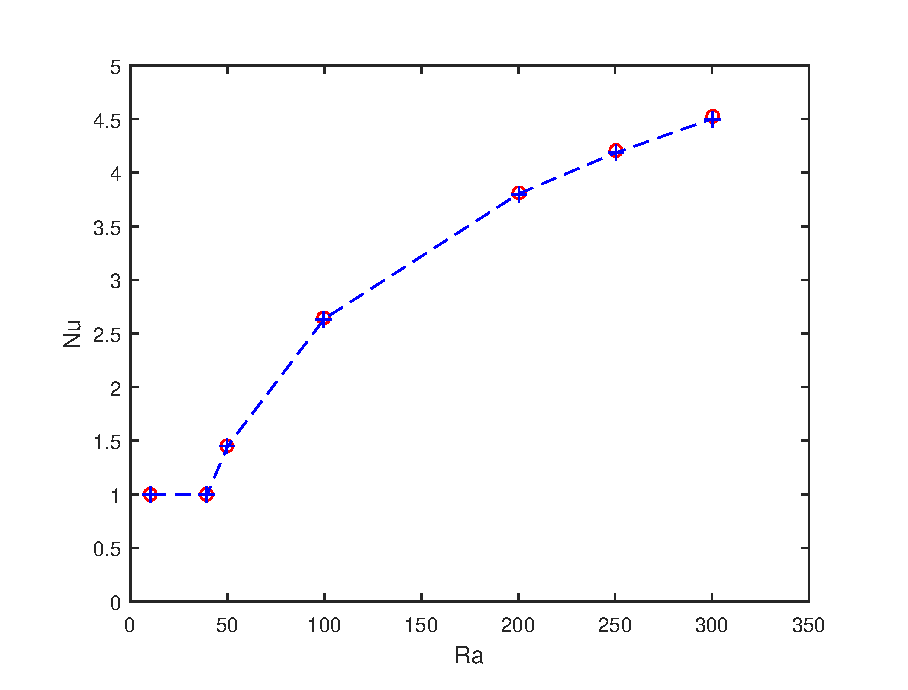
\includegraphics[width = \textwidth]{HRL-Nu-comparison}
\caption{The Horton-Rogers-Lapwood problem was solved as a further test of the code; here I plot Nu(Ra). The well documented onset of convection was observed at $4 \pi^2$, and the calculated values (blue crosses) were in good agreement with those of~\citet*{caltagirone-75} (red circles).} 
\label{fig:HRL-Nu-comparison}
\end{subfigure}
\caption{Verification of the numerical method through solving problems with known solutions.}
\label{fig:code-verification}
\end{figure}


The equations governing $\theta$ and $\psi$ within the mushy layer were solved iteratively using second order finite differences on a fixed grid. The momentum equation~\eqref{eq:momentum-simplified} was solved by successive over-relaxation (SOR)~\citep*{young-50}, whilst the time dependent heat equation~\eqref{eq:heat-psi} was solved using an Alternating Direction Implicit (ADI) method~\citep*{peaceman-rachford-55} which ensures second order temporal accuracy. A steady state was deemed to have been reached once the condition
\begin{equation}
\text{max}\left( \frac{d\theta}{dt}, \frac{d\psi}{dt}, \frac{d a}{dt} \right) < 10^{-5}
\end{equation}
was satisfied.

The mixed and Neumann boundary conditions were enforced using a Taylor expansion centered on the grid point adjacent to the boundary in order to maintain second order finite differencing. Further details of the numerical method can be found in Appendix~\autoref{app:numerical-method}.

The numerical method was implemented in MATLAB, and the code was written in stages of increasing complexity in order to verify it's accuracy. Similarity solutions for an axisymmetric heated wire are presented in ~\citet*[Chapter~5.9]{nield-bejan-06}, using which I verified second order convergence of my code when solving the system
\begin{eqnarray}
&&(\psi_r/r)_r = -R_m \theta_r; \hspace{5ex} \psi_r \theta_z - \psi_z \theta_r = (r \theta_r)_r \\
&&\theta = z \hspace{5ex} u_r = 0 \hspace{5ex} (r=a) \\
&&\theta = 0 \hspace{5ex} u_z = 0 \hspace{5ex} (r=\infty)
\end{eqnarray}
as demonstrated in figure~\ref{fig:heated-wire-error}.

In order to test both the implementation of Neumann boundary conditions and the coupling of the heat and momentum equations, I also solved the Horton-Rogers-Lapwood problem~\citep*{horton-rogers-45,lapwood-48}. I observed the onset of convection at $\text{Ra} = 4 \pi^2$, and found my results for $\text{Nu(Ra)}$ to be in good agreement with those of~\citet*{caltagirone-75} over a wide range of Ra (see figure~\ref{fig:HRL-Nu-comparison}).

Finally, once the full set of boundary conditions were applied, the steady state was checked to ensure both the interior equations and boundary conditions were satisfied.

\subsection{Free boundaries}

The full problem of steady state convection in a mushy layer, as shown in figure~\ref{fig:arrangement}, has two free boundaries which need to be determined; the chimney wall and mush-ocean interface. Whilst in reality both of these boundaries are curves, I make the simplifying assumption that they are straight sided and therefore only have to solve for their position. A known problem with the 'flat-top' approximation is that it introduces a singularity at the point where the chimney and ocean meet~\citep*{schulze-worster-98}, but this issue appears to remain localised so is accepted as a necessary compromise.

The mush-ocean boundary is treated in a subtly different way to previous authors.~\citet*{chung-worster-02} have shown that this boundary is an isotherm where
\begin{equation}
\mathbf{n} \cdot \nabla \theta = \theta_\infty \left( \nabla \cdot \mathbf{n} - \mathbf{q} \cdot \mathbf{n} \right)
\end{equation}
which in the case of a flat boundary $\mathbf{n} = \mathbf{\hat{z}}$ becomes
\begin{equation}
\theta_z = \theta_\infty (1-\psi_r / r)
\end{equation}
Instead of fixing $\theta_\infty$ and using this condition to determine $z=H$, I fix $H$ and then calculate $\theta_\infty$ from the resulting steady state. This approach removes the need to adjust the boundary at each time step, simplifying the model and reducing the runtime.

\begin{figure}[t!]
\centering
\begin{subfigure}[t]{.48\linewidth}
       \centering
       \includegraphics[width=\textwidth]{q-dot-grad-theta}
       \caption{Example cross section of $ \mathbf{q} \cdot \nabla \theta$, taken at $z=-\sfrac{2H}{3}$ for the parameters...}
       \label{fig:q-dot-grad-theta}
\end{subfigure}
\quad
\begin{subfigure}[t]{.48\linewidth}
       \centering
       \includegraphics[width=\textwidth]{q-dot-grad-theta-root}
       \caption{$ \left. \mathbf{q} \cdot \nabla \theta \right|_{r=a}$ calculated for steady state solutions with $a=b$. The negative gradient at the root $ \left. \mathbf{q} \cdot \nabla \theta \right|_{r=a} = 0$ motivates the implementation of the relaxation method~\eqref{eq:relaxation-q-dot-grad-theta}.}
    \label{fig:q-dot-grad-theta-root}
\end{subfigure}

\caption{Plots illustrating the problem of determining the free boundary $r=a$. [Placeholder plots until I make nicer ones]}
\label{fig:free-boundary-method}  

\end{figure}

Determination of the chimney wall posed significant difficulty.~\citet*{schulze-worster-99} showed, through thermodynamic considerations and the requirement that the solid fraction must be positive in the mushy layer, that  $\mathbf{q} \cdot \nabla \theta = 0$ at the chimney wall $r=a$. This condition is applied at the point $z = - \sfrac{H}{3}$ where it is expected that the straight sided approximation is most accurate; near the solid-mush boundary the chimney width is observed to decrease and may in fact disappear altogether, whilst the singularity at the mush-ocean boundary leads to unreliable values of $\theta$ and $\psi$ in the mushy layer. To enforce this condition, it is necessary to extrapolate from $r=b$ at each time step and then adjust $a$ appropriately. 

A first attempt was made using a linear extrapolation for $f(r) = \mathbf{q} \cdot \nabla \theta$
\begin{equation}
f(a) = f(b) + (a-b) \left. \frac{\partial f}{\partial r}\right|_b
\end{equation}
and solving for the root $f(a)=0$ to find a new estimate for the chimney width $a^*$ with which the chimney width $a(t)$ was updated by relaxation
\begin{equation}
\frac{da}{dt} = \lambda (a - a^*)
\end{equation}
However this produced an unstable scheme in which the chimney width became zero, as the extrapolation was highly sensitive to the position of $b$ on the $\mathbf{q} \cdot \nabla \theta$ curve (see figure~\ref{fig:q-dot-grad-theta}).

A more careful analysis revealed that, based on the form of $\psi$ and $\theta$ in the region $a < r < b$ derived in~\autoref{sec:patching-equations}, the Pad\'{e} approximation
\begin{equation}
\mathbf{q} \cdot \nabla \theta \approx \frac{a r^3 + b r^2 + c r + d}{r}
\end{equation}
would be more appropriate. However this too was found to be unstable, in this case due to the $\sfrac{1}{r}$ term causing the extrapolation to, in some cases, predict no roots at all.

Removing the $\sfrac{1}{r}$ term and instead considering a quadratic function was slightly more successful, but the predicted chimney widths $a^*$ were still highly dependant on the form of $\mathbf{q} \cdot \nabla \theta$ at $r=b$ and convergence to a steady state with chimneys could not be achieved.

By fixing $a=b$ and finding steady states at a range of chimney widths, it was observed that $\left. \mathbf{q} \cdot \nabla \theta \right|_{r=a}$ approaches a root from above (see figure~\ref{fig:q-dot-grad-theta-root}). Therefore a new relaxation scheme was employed
\begin{equation}
\label{eq:relaxation-q-dot-grad-theta}
\frac{da}{dt} = \lambda \left. \mathbf{q} \cdot \nabla \theta \right|_{r=a}
\end{equation}
where $\left. \mathbf{q} \cdot \nabla \theta \right|_{r=a}$ was calculated using a quadratic extrapolation from $r=b$ and $\lambda = 0.002$. Using this method it was possible to converge on a steady state with chimneys, so the description of the numerical scheme is complete.

\begin{figure}[ht!]
\centering
\begin{subfigure}[t]{.48\linewidth}
    \centering
    \includegraphics[width=0.9\textwidth]{steady-state-Rm60H0-25R0-25}
    \caption{Streamlines in the reference frame of the solid phase}
    \label{fig:steady-state-darcy}
 \end{subfigure}
 \quad
 \begin{subfigure}[t]{.48\linewidth}
    \centering
    \includegraphics[width=0.9\textwidth]{steady-state-Rm60H0-25R0-25-q}
    \caption{Streamlines in the laboratory reference frame}
    \label{fig:steady-state-q}
 \end{subfigure}
    
    \caption{Steady state temperature and flow fields for $Rm=60, R=0.25, H=0.25, Da=5\times10^{-5}$. Dashed black lines are contours of equal $\theta$, ranging from $\theta=-1$ at $z=0$ to $\theta=0$ at $z=-H$ in $0.1$ increments. Solid blue lines are streamlines [need to work out the range and interval of psi]. In figure (a) these are streamlines of the Darcy velocity $\mathbf{u}$, whilst in figure (b) they are calculated from $\mathbf{q} = \mathbf{u} + V \mathbf{\hat{z}}$. The red vertical line illustrates the position of the chimney wall, $a$.}
    \label{fig:typical-steady-states}
 \end{figure}

\section{Results and their interpretation}
\label{sec:results}


 
 
 
  \begin{figure}[ht!]
\centering
\begin{subfigure}[t]{.48\linewidth}
    \centering
    \includegraphics[width=\textwidth]{Rm-a-H0-25R0-34}
    \caption{}
    \label{fig:steady-state-Rm-a}
 \end{subfigure}
 \quad
 \begin{subfigure}[t]{.48\linewidth}
    \centering
    \includegraphics[width=\textwidth]{Rm-flux-H0-25R0-34}
    \caption{}
    \label{fig:steady-state-Rm-flux}
 \end{subfigure}
\quad
  \begin{subfigure}[t]{.48\linewidth}
    \centering
    \includegraphics[width=\textwidth]{Rm-theta-inf-H0-25R0-34}
    \caption{}
    \label{fig:steady-state-Rm-theta-inf}
 \end{subfigure}
  \quad
 \begin{subfigure}[t]{.48\linewidth}
    \centering
    \includegraphics[width=\textwidth]{Rm-psi-H0-25R0-34}
    \caption{}
    \label{fig:steady-state-Rm-psi}
 \end{subfigure}
 
 \caption{Plots of (a) chimney width, (b) flux at the solid-mush boundary (c) $\theta_\infty$ and (d) $\psi_{max}$ as a function of Rm for $R=0.25, H=0.34, Da=5\times10^{-5}$. Below $\text{Rm} = 47$ no steady states were found with non-zero $a$.}
 \label{fig:parameter-plots}
 \end{figure}



The numerical method, whilst stable, requires $(b-a) \ll a$. This makes finding steady states for arbitrary parameters impossible, as a very good first guess for $a$ is required. An initial steady state was found for the parameters $Rm = 60, R=0.25, H=0.25, Da=5\times 10^{-5}$ by bracketing a root of $\left. \mathbf{q} \cdot \nabla \theta \right|_{r=a} = 0$, and each parameter was then varied by small amounts ($\sim 1\%$ of their value) such that the previous value of $a$ was a good estimate for the new state. This allowed for a range of parameter space to be explored.

A typical steady state is shown in figure~\ref{fig:typical-steady-states}, where the solution has been extended into $0 \le r \le b$ using the approximate solutions derived in~\autoref{sec:approximations}. The singularity resulting from the straight mush-ocean boundary can be clearly seen by it's distorting effect on the extrapolated values in the chimney region. However the affected region is small relative to the whole domain, so should not affect the overall form of the solution. The parallel isotherms and streamlines at $(r, z) = (a, -\sfrac{2H}{3})$ in figure~\ref{fig:steady-state-q} confirm that the condition $\left. \mathbf{q} \cdot \nabla \theta \right|_{r=a} = 0$, used to determine the position of the chimney wall, is indeed satisfied. Comparison between figures~\ref{fig:steady-state-darcy} and~\ref{fig:steady-state-q} illustrates the difference between viewing the system in a frame of reference fixed to the solid-mush boundary (a) and in laboratory frame (b) and. In the latter case, fluid flow enters the solid with vertical velocity $V$, the solidification rate (NOTE - currently can't get MATLAB to plot the streamlines that the leave mushy region into the solid, so figure~\ref{fig:steady-state-q} doesn't actually show this). Due to the (relatively) large Rayleigh number, these parameters are significantly different to those for which previous authors have produced similar plots making direct comparison of results difficult. However the general features are seen to be in good agreement with figure 5(c) from~\citet*{schulze-worster-98}.

By varying Rm at fixed $R$ and $H$~\cref{fig:steady-state-Rm-a,fig:steady-state-Rm-flux,fig:steady-state-Rm-theta-inf,fig:steady-state-Rm-psi} were produced. Fluxes at the solid-mush boundary, $F_s$, were found using the calculation described in~\cref{app:heat-flux} (NOTE: this graph doesn't seem right, need to check the calculation). I have not been able to continue the curves backwards beyond $\text{Rm} = 47$, where studies by previous authors suggest there should exist a set of unstable states forming the lower branch of a saddle point bifurcation~\citep*{schulze-worster-98,chung-worster-02}. Instead, the numerical method jumps to steady states with no chimney, $a=0$, which are not of interest. [Need to make more of an effort to see if I can get to the lower branch by reducing Rm in smaller steps or decreasing $\Delta r$ before deciding it's impossible and offering possible explanations for why the model cannot get to it].

\begin{figure}[hb!]
 \begin{subfigure}[t]{.48\linewidth}
   \centering
   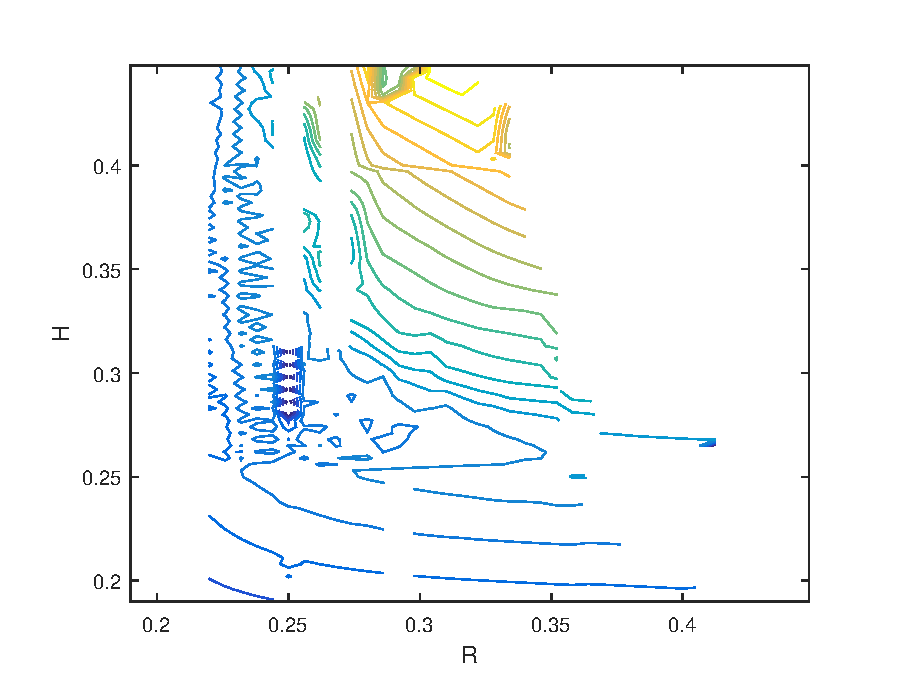
\includegraphics[width=0.8\textwidth]{R-H-psi-max}
   \caption{}
   \label{fig:R-H-psi-max}   
\end{subfigure}
\quad
\begin{subfigure}[t]{.48\linewidth}
   \centering
   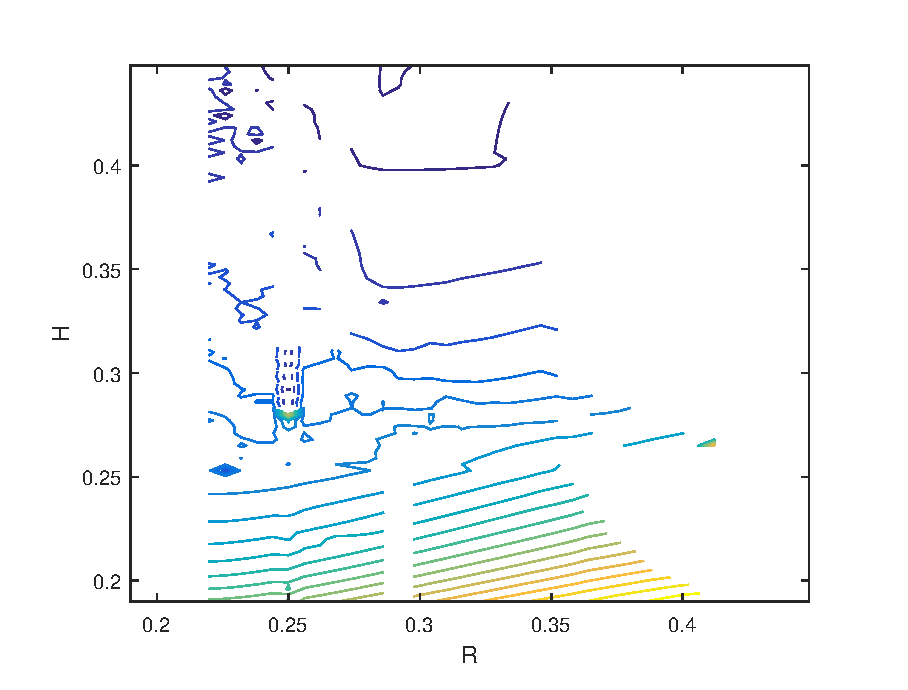
\includegraphics[width=0.8\textwidth]{R-H-theta-inf}
   \caption{}
   \label{fig:R-H-theta-inf}   
\end{subfigure}

\caption{Contour plot of (a) $\psi_{max}$ and (b) $\theta_\infty$ in the $R-H$ plane for $\text{Rm} = 60, Da=5\times10^{-5}$. Currently incomplete data.}
\label{fig:R-H-contour}
 
\end{figure} 
[I would also like to investigate the dependence on $R$ of the Rayleigh number at which the chimney disappears, and produce some contour plots of $R-H$ space (e.g.~\cref{fig:R-H-contour}), but at the moment don't have enough data to draw any sensible conclusions]


\section{Conclusion}
\label{sec:conclusion}
I have derived and solved a model for steady convection in an ideal mushy layer, using a two dimensional axisymmetric geometry with a periodic array of brine channels. Through a suitable choice of boundary conditions I avoided the computationally intensive problem of solving for the fluid flow in the ocean and the chimney. The governing equations within the mushy layer were simplified through a catalogue of assumptions which, most importantly, removed the dependence on permeability and decoupled the equations for conservation of heat and solute. Meanwhile the geometry was simplified by the assumption that the convection cell has straight edges. The free boundary problem for the chimney wall was solved using relaxation based on the condition derived by~\citet*{schulze-worster-99}. The equivalent problem for the mush-ocean interface was eliminated by fixing $H$ for each steady state, at the expense of relinquishing control over the parameter determining the far field temperature in the ocean, $\theta_\infty$.

Despite the significant approximations imposed, the model still produces steady state temperature and velocity profiles in broad agreement with those published by other authors using more complex methods. Direct numerical comparison of results is made difficult by my choice of parameters, which were necessary in order to find converging solutions. 

[Can't add any more specific details about the results and their consequences until I have them/have analysed them]

The most significant source of error in the model is the flat boundary applied at the mush-ocean interface and consequent singularity at the point where this boundary meets the chimney. Applying a functional form for $H = H(r)$ that satisfies the boundary conditions on $\theta$, as~\citet*{schulze-worster-98} did in a planar geometry, would be a sensible next step to improve this model. Doing so would require the re-mapping of the domain in the vertical direction, but would produce more reliable numerical results for comparison with other studies.

\newpage
\bibliography{references}{}








%%%%%%%%%%%%%%%%%%%%%%%%%%%%%%%%%%%%%%%%%%%%%
%%%%%%%%%%%%%%%%%%%%%%%%%%%%%%%%%%%%%%%%%%%%%
%%%%%%%%%%%%%%             Appendix         %%%%%%%%%%%%%%%%%%%%%
%%%%%%%%%%%%%%%%%%%%%%%%%%%%%%%%%%%%%%%%%%%%%
%%%%%%%%%%%%%%%%%%%%%%%%%%%%%%%%%%%%%%%%%%%%%
\newpage
\appendix
\label{appendix}

\section{Numerical method}
\label{app:numerical-method}
To-do. \\
More details on the ADI scheme, coupling of the equations, discretization, and a link to where the code can be found.

\section{Heat flux}
\label{app:heat-flux}
The heat equation can be written
\begin{equation}
\frac{\partial \theta}{\partial t} + \nabla \cdot \left[ \mathbf{q} \theta - \nabla \theta \right] = 0
\end{equation}
so in steady state, using the divergence theorem,
\begin{equation}
\int_V \nabla \cdot \left[ \mathbf{q} \theta - \nabla \theta \right] dV = \oiint_S \left[ \mathbf{q} \theta - \nabla \theta \right] \cdot \mathbf{\hat{n}} \; dS = 0
\end{equation}
The net heat fluxes out of the convection cell balance. Furthermore, the boundary conditions ensure there is no heat flux from $r=0, R$.

I am interested in the heat flux from the mush to the solid, at $z=0$, given by
\begin{equation}
F_{s} = \frac{1}{\pi R^2} \int_{r=0}^R \left( \mathbf{q}.\mathbf{n} \theta + \frac{\partial \theta}{\partial z} \right) 2 \pi r \; dr \hspace{5ex} (z=0)
\end{equation}
There is no normal flow at this boundary, $\theta=-1$ and $\mathbf{n} = \mathbf{\hat{z}}$. For $r<b$, I use the approximation $\left. \theta_z \right|_{r<b} = \left. \theta_z \right|_{r=b}$. Therefore
\begin{equation}
F_{s} = - 1  + \left( \frac{b}{R} \right)^2 \left.  \frac{\partial \theta}{\partial z} \right|_{r=b} + \frac{1}{\pi R^2} \int_{r=b}^R  \frac{\partial \theta}{\partial z}  2 \pi r \; dr
\end{equation}
The integral is carried out numerically with the MATLAB function \texttt{trapz}.




\end{document}